\documentclass{report}
\input{preamble.tex}
\usepackage{circuitikz}
\usepackage[scr]{rsfso}
\usetikzlibrary{circuits.ee.IEC}
\usetikzlibrary{arrows,shapes.gates.logic.US,shapes.gates.logic.IEC,calc}
\newcommand{\faketarget}{\oplus\!\!\!\!\odot}
\newcommand{\target}{%
  
\begin{tikzpicture}[scale=0.5]
    \fill[black] (0,0) circle (0.1);
    \draw (0,0) circle (0.2);
    \draw (0,0) circle (0.3);
  \end{tikzpicture}%
}

\usepackage[clock]{ifsym}
\usepackage{karnaugh-map}


\title{\Huge{Architecture des ordinateurs}\\{IFT1227}\\{\textbf{Introduction}}}
\author{\huge{Franz Girardin}}
\date{\today}
\lstset{inputencoding=utf8/latin1}

            %%%%%%%%%%%%%%%%%  Sect.                          %%%%%%%%%%%%%%%%%%%%%%%%%%%%%%%%%%%%%%%%%%%%%%%%%%%%%%%%%
\usepackage{helvet}
\titleformat{\chapter}
  {\fontfamily{phv}\bfseries\huge} % format
  {}                % label
  {0pt}             % sep
  {\color{myb}\huge}           % before-code



\titleformat{\section}
  {\normalfont\scshape}{\thesection}{1em}{}
\usepackage{circuitikz}


% Customizing the spacing for the chapter titles
\titlespacing*{\chapter}{0pt}{0pt}{20pt}

% Allow hfill in math environment
\newcommand{\specialcell}[1]{\ifmeasuring@#1\else\omit$\displaystyle#1$\ignorespaces\fi}

% Allow you to do the non implication (implication barred)
\newcommand{\notimplies}{%
  \mathrel{{\ooalign{\hidewidth$\not\phantom{=}$\hidewidth\cr$\implies$}}}}



\DeclareRobustCommand{\looongrightarrow}{%
  \DOTSB\relbar\joinrel\relbar\joinrel\relbar\joinrel\rightarrow
}



% Define the command for the NOT gate
\newcommand{\notgate}{%
    \begin{circuitikz}[scale=0.8, transform shape]
        \draw
        (0,0) node[not port] (mynot) {}
        (mynot.in) -- ++(-0.5,0) node[left] {A}
        (mynot.out) -- ++(0.5,0) node[right] {Y};
    \end{circuitikz}
}


\newcommand{\bufgate}{%
    \begin{circuitikz}[scale=0.8, transform shape]
        \draw
        (0,0) node[buffer port] (mynot) {}
        (mynot.in) -- ++(-0.5,0) node[left] {A}
        (mynot.out) -- ++(0.5,0) node[right] {Y};
    \end{circuitikz}
}



\newcommand{\andgate}{%
    \begin{circuitikz}[scale=0.8, transform shape]
        \draw
        (0,0) node[and port] (myand) {}
        (myand.in 1) -- ++(-0.5,0) node[left] {A}
        (myand.in 2) -- ++(-0.5,0) node[left] {B}
        (myand.out) -- ++(0.5,0) node[right] {Y};
    \end{circuitikz}
}


% Define the command for the OR gate
\newcommand{\orgate}{%
    \begin{circuitikz}[scale=0.8, transform shape]
        \draw
        (0,0) node[or port] (myor) {}
        (myor.in 1) -- ++(-0.5,0) node[left] {A}
        (myor.in 2) -- ++(-0.5,0) node[left] {B}
        (myor.out) -- ++(0.5,0) node[right] {Y};
    \end{circuitikz}
}


% Define the command for the XOR gate
\newcommand{\xorgate}{%
    \begin{circuitikz}[scale=0.8, transform shape]
        \draw
        (0,0) node[xor port] (myxor) {}
        (myxor.in 1) -- ++(-0.5,0) node[left] {A}
        (myxor.in 2) -- ++(-0.5,0) node[left] {B}
        (myxor.out) -- ++(0.5,0) node[right] {Y};
    \end{circuitikz}
}

% Define the command for the NOR gate
\newcommand{\norgate}{%
    \begin{circuitikz}[scale=0.8, transform shape]
        \draw
        (0,0) node[nor port] (mynor) {}
        (mynor.in 1) -- ++(-0.5,0) node[left] {A}
        (mynor.in 2) -- ++(-0.5,0) node[left] {B}
        (mynor.out) -- ++(0.5,0) node[right] {Y};
    \end{circuitikz}
}

% Define the command for the NAND gate
\newcommand{\nandgate}{%
    \begin{circuitikz}[scale=0.8, transform shape]
        \draw
        (0,0) node[nand port] (mynand) {}
        (mynand.in 1) -- ++(-0.5,0) node[left] {A}
        (mynand.in 2) -- ++(-0.5,0) node[left] {B}
        (mynand.out) -- ++(0.5,0) node[right] {Y};
    \end{circuitikz}
}

% Define the command for the XNOR gate
\newcommand{\xnorgate}{%
\begin{circuitikz}[scale=0.8, transform shape]
\draw
(0,0) node[xnor port] (myxnor) {}
(myxnor.in 1) -- ++(-0.5,0) node[left] {A}
(myxnor.in 2) -- ++(-0.5,0) node[left] {B}
(myxnor.out) -- ++(0.5,0) node[right] {Y};
\end{circuitikz}
}


% Define the command for the 3-input NOR gate
\newcommand{\northreegate}{%
    \begin{circuitikz}[scale=0.8, transform shape]
        \draw
        (0,0) node[nor port, number inputs=3] (mynor3) {}
        (mynor3.in 1) -- ++(-0.5,0) node[left] {A}
        (mynor3.in 2) -- ++(-0.5,0) node[left] {B}
        (mynor3.in 3) -- ++(-0.5,0) node[left] {C}
        (mynor3.out) -- ++(0.5,0) node[right] {Y};
    \end{circuitikz}
}


% Define the command for the 3-input AND gate
\newcommand{\andthreegate}{%
\begin{circuitikz}[scale=0.8, transform shape]
    \draw
    (0,0) node[and port, number inputs=3] (myand3) {}
    (myand3.in 1) -- ++(-0.5,0) node[left] {A}
    (myand3.in 2) -- ++(-0.5,0) node[left] {B}
    (myand3.in 3) -- ++(-0.5,0) node[left] {C}
    (myand3.out) -- ++(0.5,0) node[right] {Y};
\end{circuitikz}

}



\begin{document}
\maketitle

\pagebreak

\pagebreak
\begin{multicols*}{3}


    \footnotesize


    \paragraph{Couche logique numérique}  
    Constituées de \textit{portes logiques} construite à partir 
    de \textbf{transisteurs} qui prennent un \textbf{signal}
    \textbf{0} ou \textbf{1} et calcule 
    une \textbf{fonction logique} 
    $\mathbb{ET}$, $\mathbb{OU}$ et $\mathbb{NON}$, etc.

    \paragraph{Porte $\mathbb{NON}$}
    \mbox{}\vspace{1em}\\
    \begin{minipage}{\columnwidth}
        \begin{minipage}[b]{0.5\columnwidth}
            \centering
            \notgate
        \end{minipage}%
        \begin{minipage}[b]{0.5\columnwidth}
            \centering
            \raisebox{0.3\height}{
            \renewcommand{\arraystretch}{1.5}
            \begin{tabular}{c|c}
                A & Y \\
                \hline
                1 & 0 \\
                0 & 1 \\
            \end{tabular}
            }
        \end{minipage}
    \end{minipage}
    \[\entouree{$Y= \overline{A}$} \]


    \paragraph{Porte $\mathbb{BUF}$}
    \mbox{}\vspace{1em}\\
    \begin{minipage}{\columnwidth}
        \begin{minipage}[b]{0.5\columnwidth}
            \centering
            \bufgate
        \end{minipage}%
        \begin{minipage}[b]{0.5\columnwidth}
            \centering
            \raisebox{0.3\height}{
            \renewcommand{\arraystretch}{1.5}
            \begin{tabular}{c|c}
                A & Y \\
                \hline
                0 & 0 \\
                1 & 1 \\
            \end{tabular}
            }
        \end{minipage}
    \end{minipage}
    \[\entouree{$Y= A$} \]



    \paragraph{Porte $\mathbb{ET}$}
    \mbox{}\vspace{1em}\\
    \begin{minipage}{\columnwidth}
        \begin{minipage}[b]{0.5\columnwidth}
            \centering
            \andgate
        \end{minipage}%
        \begin{minipage}[b]{0.5\columnwidth}
            \centering
            \raisebox{-0.3\height}{
            \renewcommand{\arraystretch}{1.5}
            \begin{tabular}{c c | c}
                A & B & Y \\
                \hline
                0 & 0 & 0 \\
                0 & 1 & 1 \\
                1 & 0 & 1 \\
                1 & 1 & 1 
            \end{tabular}
            }
        \end{minipage}
    \end{minipage}
    \[\entouree{$Y = AB $} \]



    \paragraph{Porte $\mathbb{OU}$}
    \mbox{}\vspace{1em}\\
    \begin{minipage}{\columnwidth}
        \begin{minipage}[b]{0.5\columnwidth}
            \centering
            \orgate
        \end{minipage}%
        \begin{minipage}[b]{0.5\columnwidth}
            \centering
            \raisebox{-0.3\height}{
            \renewcommand{\arraystretch}{1.5}
            \begin{tabular}{c c | c}
                A & B & Y \\
                \hline
                0 & 0 & 0 \\
                0 & 1 & 0 \\
                1 & 0 & 0 \\
                1 & 1 & 1 
            \end{tabular}
            }
        \end{minipage}
    \end{minipage}
    \[\entouree{$Y = A + B $} \]



    \paragraph{Porte $\mathbb{XOR}$}
    \mbox{}\vspace{1em}\\
    \begin{minipage}{\columnwidth}
        \begin{minipage}[b]{0.5\columnwidth}
            \centering
            \xorgate
        \end{minipage}%
        \begin{minipage}[b]{0.5\columnwidth}
            \centering
            \raisebox{-0.3\height}{
            \renewcommand{\arraystretch}{1.5}
            \begin{tabular}{c c | c}
                A & B & Y \\
                \hline
                0 & 0 & 0 \\
                0 & 1 & 1 \\
                1 & 0 & 1 \\
                1 & 1 & 0 
            \end{tabular}
            }
        \end{minipage}
    \end{minipage}
    \[\entouree{$Y = A \oplus B$} \]
    \columnbreak



    \paragraph{Porte $\mathbb{NAND}$}
    \mbox{}\vspace{1em}\\
    \begin{minipage}{\columnwidth}
        \begin{minipage}[b]{0.5\columnwidth}
            \centering
            \nandgate
        \end{minipage}%
        \begin{minipage}[b]{0.5\columnwidth}
            \centering
            \raisebox{-0.3\height}{
            \renewcommand{\arraystretch}{1.5}
            \begin{tabular}{c c | c}
                A & B & Y \\
                \hline
                0 & 0 & 1 \\
                0 & 1 & 1 \\
                1 & 0 & 1 \\
                1 & 1 & 0 
            \end{tabular}
            }
        \end{minipage}
    \end{minipage}
    \[\entouree{$Y = \overline{AB}$} \]


    \paragraph{Porte $\mathbb{NOR}$}
    \mbox{}\vspace{1em}\\
    \begin{minipage}{\columnwidth}
        \begin{minipage}[b]{0.5\columnwidth}
            \centering
            \norgate
        \end{minipage}%
        \begin{minipage}[b]{0.5\columnwidth}
            \centering
            \raisebox{-0.3\height}{
            \renewcommand{\arraystretch}{1.5}
            \begin{tabular}{c c | c}
                A & B & Y \\
                \hline
                0 & 0 & 1 \\
                0 & 1 & 0 \\
                1 & 0 & 0 \\
                1 & 1 & 0 
            \end{tabular}
            }
        \end{minipage}
    \end{minipage}
    \[\entouree{$Y = \overline{A + B}$} \]



    \paragraph{Porte $\mathbb{XNOR}$}
    \mbox{}\vspace{1em}\\
    \begin{minipage}{\columnwidth}
        \begin{minipage}[b]{0.5\columnwidth}
            \centering
            \xnorgate
        \end{minipage}%
        \begin{minipage}[b]{0.5\columnwidth}
            \centering
            \raisebox{-0.3\height}{
            \renewcommand{\arraystretch}{1.5}
            \begin{tabular}{c c | c}
                A & B & Y \\
                \hline
                0 & 0 & 1 \\
                0 & 1 & 0 \\
                1 & 0 & 0 \\
                1 & 1 & 1 
            \end{tabular}
            }
        \end{minipage}
    \end{minipage}
    \[\entouree{$Y = \overline{A \oplus B}$} \]



    \paragraph{Porte $\mathbb{NOR}3$}
    \mbox{}\vspace{1em}\\
    \begin{minipage}{\columnwidth}
        \begin{minipage}[b]{0.5\columnwidth}
            \centering
            \northreegate
        \end{minipage}%
        \begin{minipage}[b]{0.5\columnwidth}
            \centering
            \raisebox{-0.6\height}{
            \renewcommand{\arraystretch}{1.5}
            \begin{tabular}{c c c | c}
                A & B & C & Y \\
                \hline
                0 & 0 & 0 & 1 \\
                0 & 0 & 1 & 0 \\
                0 & 1 & 0 & 0 \\
                0 & 1 & 1 & 0 \\
                1 & 0 & 0 & 0 \\
                1 & 0 & 1 & 0 \\
                1 & 1 & 0 & 0 \\
                1 & 1 & 1 & 0 
            \end{tabular}
            }
        \end{minipage}
    \end{minipage}
    \[\entouree{$Y = \overline{A + B + C}$} \]
    \columnbreak



    \paragraph{Porte $\mathbb{AND}3$}
    \mbox{}\vspace{1em}\\
    \begin{minipage}{\columnwidth}
        \begin{minipage}[b]{0.5\columnwidth}
            \centering
            \andthreegate
        \end{minipage}%
        \begin{minipage}[b]{0.5\columnwidth}
            \centering
            \raisebox{-0.6\height}{
            \renewcommand{\arraystretch}{1.5}
            \begin{tabular}{c c c | c}
                A & B & C & Y \\
                \hline
                0 & 0 & 0 & 0 \\
                0 & 0 & 1 & 0 \\
                0 & 1 & 0 & 0 \\
                0 & 1 & 1 & 0 \\
                1 & 0 & 0 & 0 \\
                1 & 0 & 1 & 0 \\
                1 & 1 & 0 & 0 \\
                1 & 1 & 1 & 1 
            \end{tabular}
        }         
    \end{minipage}
    \end{minipage}
    \[\entouree{$Y = ABC$} \]

    \paragraph{Définition de la marge de bruit}
    Tolérance d'un circuit aux \textbf{perturbations} 
    pouvant fausser l'interprétation du signal.  
    \begin{itemize}
        \item[$\rhd$] $ V_{IH}$ : $\min(V | V_{in}\Coloneqq \textbf{1})$  
        \item[$\rhd$]  $V_{IL}$ : $\max(V | V_{in}\Coloneqq \textbf{0})$
        \item[$\blacktriangleright$] Signal reçu \textbf{min} ou \textbf{max} 
            est être interprété comme \textbf{1}  ou \textbf{0}. 
        \item[$\rhd$] $ V_{OH}$ : $\min(V | V_{out}\Coloneqq \textbf{1})$  
        \item[$\rhd$] $V_{OL}$ : $\max(V | V_{out}\Coloneqq \textbf{0})$
        \item[$\blacktriangleright$] Signal \textbf{min} ou \textbf{max} 
            que l'émetteur s'engage à fournir pour être interprété 
            comme \textbf{1}  ou \textbf{0}. 
    \end{itemize}
    \begin{align*}
        NM_H = V_{OH} \; (\textit{ém.}) - V_{IH} \; (src.) \\
        NM_L = V_{IL} (src.) - V_{OL} (\textit{ém.})
    \end{align*}

    \begin{figure}[H]
        \begin{center}
            \includegraphics[width=0.30\textwidth]{MargeBruit.png}
        \end{center}
    \end{figure}

    \paragraph{Transistors}
    \mbox{}\vspace{1em}\\
    Éléments de base des circuits électroniques. Ils sont composés de 
    trois broches; le drain, la source, et la \textbf{grille} qui contrôle 
    les deux autres comme un interrupteur.  La figure suivante représente 
    un transistor hors tension \textit{off}, un transistor hors tension 
    mais polarisé \textit{off} et un transistor sous tension \textit{on}.     
    \begin{center}
    \begin{circuitikz}[scale=0.5]
    % Draw NMOS transistor
    \draw (0,0) node[nigfete] (mos) {}
    (mos.gate) node[left] {g}
    (mos.drain) node[above] {d}
    (mos.source) node[below] {s};

    % Draw NMOS in OFF state
    \draw (3,0) node[nigfete] (mosoff) {}
    (mosoff.gate) node[left] {g}
    (mosoff.drain) node[above] {d}
    (mosoff.source) node[below] {s};
    \draw (mosoff.gate) -- ++(0.5,0) node[circ] {} -- (mosoff.source);

    Draw NMOS in ON state
    \draw (6,0) node[nigfete] (moson) {}
    (moson.gate) node[left] {g}
    (moson.drain) node[above] {d}
    (moson.source) node[below] {s};
    \draw (moson.gate) -- ++(0.5,0) node[circ] {} -- (moson.drain);
    \end{circuitikz}
    \end{center}

    \paragraph{Composition d'un circuit} 
    \mbox{}\\ 
    \textbf{Circuit}$\Coloneqq$ E., S., spec. \textit{fonct}., spec. \textit{temp}.   

    \paragraph{Propriétés d'un circ. combinatoire}
    \mbox{} 
    \vspace{0.1em}
    \begin{itemize}
        \item[$\rhd$]  \textbf{Noeud} $\implies$ \textit{In}  
            ou \textbf{connexion à} un \textit{Out}. 
        \item[$\rhd$] \textbf{Aucun} chemin cyclique.    

    \end{itemize}


    \paragraph{Sommes de produits SOP}
    En considérant les variables \textit{In} d'une ligne de la table de vérité, 
    il faut identifier la \textbf{conjonction} (produit) nécessaire 
    pour engendrer un \textbf{1} logique. Un \textbf{minterm} est une 
    représentation du produit engendrant un 1 logique. 

                \begin{table}[H]
                  \begin{center}
                   \renewcommand{\arraystretch}{1.5}
                    \footnotesize
                        \begin{tabular}{|l|l|l||c|}
                        \arrayrulecolor{blue}\hline
                        \rowcolor{lightBlue}
                        \textcolor{myb}{$A$} & \textcolor{myb}{$B$} 
                                           & \textcolor{myb}{$Y$} 
                                           & \textcolor{myb}{\textit{minterm}}  
                        \\
                        \hline
                        \hline
                        \arrayrulecolor{black}
                        $V$ & $F$ & \cellcolor{myr} $0$ & $\overline{AA}$
                        \\
                        \hline
                        $0$ & $1$ & \cellcolor{myg} $1$ & \textcolor{myg}{$\overline{A}B$}
                        \\
                        \hline 
                        $1$ & $0$ & \cellcolor{myr} $0$ & $A\overline{B}$ 
                        \\ 
                        \hline
                        $1$ & $1$ & \cellcolor{myg} $1$ & \textcolor{myg}{$AB$}
                        \\
                        \hline
                        \end{tabular}
                \end{center}
                \end{table}
                \[Y(A, B) = \overline{A}B + AB \leftrightarrow Y(A,B) = \sum (1, 3) \]
    

    \paragraph{Produits de sommes}
    En considérant les variables \textit{In} d'une ligne de la table de vérité, 
    il faut identifier la \textbf{somme} nécessaire 
    pour engendrer un \textbf{0} logique. Un \textbf{maxterm} est une 
    représentation de la somme engendrant un 0 logique. 


                \begin{table}[H]
                  \begin{center}
                   \renewcommand{\arraystretch}{1.5}
                     \footnotesize
                        \begin{tabular}{|l|l|l||c|}
                        \arrayrulecolor{blue}\hline
                        \rowcolor{lightBlue}
                        \textcolor{myb}{$A$} & \textcolor{myb}{$B$} 
                                           & \textcolor{myb}{$Y$} 
                                           & \textcolor{myb}{\textit{maxterm}}  
                        \\
                        \hline
                        \hline
                        \arrayrulecolor{black}
                        $V$ & $F$ & \cellcolor{myg} $0$ & \textcolor{myg}{$A + B$}
                        \\
                        \hline
                        $0$ & $1$ & \cellcolor{myr} $1$ & $A + \overline{B}$
                        \\
                        \hline 
                        $1$ & $0$ & \cellcolor{myg} $0$ & \textcolor{myg}{$\overline{A} + B$} 
                        \\ 
                        \hline
                        $1$ & $1$ & \cellcolor{myr} $1$ & $\overline{A} + \overline{B}$ 
                        \\
                        \hline
                        \end{tabular}
                \end{center}
                \end{table}
                \[Y(A, B) = (A+B)(A + \overline{B}) = \prod (0, 2) \]



    \begin{table}[H]
      \centering
      \renewcommand{\arraystretch}{1.5}
      \setlength{\arrayrulewidth}{0.4pt}
      \arrayrulecolor{blue}
      \scriptsize
      \begin{tabular}{|l|l|l|}
        \hline
        \rowcolor{lightBlue}
        \textcolor{myb}{Axiome} & \textcolor{myb}{Dual} & \textcolor{myb}{Nom} \\
        \hline
        \hline
        \( B = 0 \) if \( B \neq 1 \) & \( B = 1 \) if \( B \neq 0 \) & Bin. field \\
        \rowcolor{lightBlue}
        \( \overline{0} = 1 \) & \( \overline{1} = 0 \) & NOT \\
        \( 0 \cdot 0 = 0 \) & \( 1 + 1 = 1 \) & AND/OR \\
        \rowcolor{lightBlue}
        \( 1 \cdot 1 = 1 \) & \( 0 + 0 = 0 \) & AND/OR \\
        \( 0 \cdot 1 \cdot 0 = 0 \) & \( 1 + 0 = 1 + 1 \) & AND/OR \\
        \hline
        \end{tabular}
    \end{table}



    \begin{table}[H]
      \centering
      \renewcommand{\arraystretch}{1.5}
      \setlength{\arrayrulewidth}{0.4pt}
      \arrayrulecolor{blue}
      \footnotesize
      \begin{tabular}{|l|l|l|}
        \hline
        \rowcolor{lightBlue}
        \textcolor{myb}{Théorème} & \textcolor{myb}{Dual} & \textcolor{myb}{Nom} \\
        \hline
        \hline
        $B \cdot 1 = B$ & $B + 0 = B$ & Identité \\
        \rowcolor{lightBlue}
        \( B \cdot  0 = 0\) & \( B + 1 = 1 \) & Élément nul \\
        \( B \cdot B = B \) & \( B + B = B \) & Indépotence \\
        \rowcolor{lightBlue}
                            & \( \overline{\overline{B}}  = B\) & Involution \\
        \( B \cdot \overline{B} = 0 \) & \( B + \overline{B} = 1 \) & Complément \\
        \hline
        \end{tabular}
    \end{table}


    \paragraph{De Morgan}
    \mbox{}\vspace{0.5em}
    \[ \neg(A + B) = \neg A + \neg B \]
    \[ \neg(A \cdot B) = \neg A \cdot \neg B \]

    \paragraph{Exemple simple de circuit combinatoire} 
    \mbox{}\vspace{0.5em}



\tikzstyle{branch}=[fill,shape=circle,minimum size=3pt,inner sep=0pt]
\begin{tikzpicture}[label distance=1mm, scale=0.75]

    \node (x0) at (0,0) {$A$};
    \node (x1) at (1,0) {$B$};
    \node (x2) at (2,0) {$C$};

    \node[not gate US, draw, rotate=-90] at ($(x2)+(0.5,-1)$) (Not2) {};
    \node[not gate US, draw, rotate=-90] at ($(x1)+(0.5,-1)$) (Not1) {};
    \node[not gate US, draw, rotate=-90] at ($(x0)+(0.5,-1)$) (Not0) {};


    \node[and gate US, draw, logic gate inputs=nnn] at ($(x2)+(2,-2)$) (And1) {};
    \node[and gate US, draw, logic gate inputs=nnn] at ($(And1)+(0,-1)$) (And2) {};
    \node[and gate US, draw, logic gate inputs=nnn] at ($(And2)+(0,-1)$) (And3) {};

    \node[or gate US, draw, rotate=-90, logic gate inputs=nnn] at ($(And3)+(1,-1)$) (Or1) {};


    \foreach \i in {0, 1, 2}
    {
        \path (x\i) -- coordinate (punt\i) (x\i |- Not\i.input);
        \draw (punt\i) node[branch] {} -| (Not\i.input);
    }




    \draw (Not0.output |- And1.input 1) node[branch] {} -- (And1.input 1);
    \draw (Not1.output |- And1.input 2) node[branch] {} -- (And1.input 2);
    \draw (Not2.output |- And1.input 3) node[branch] {} -- (And1.input 3);

    \draw (x0 |- And2.input 1) node[branch] {} -- (And2.input 1);
    \draw (Not1.output |- And2.input 2) node[branch] {} -- (And2.input 2);
    \draw (Not2.output |- And2.input 3) node[branch] {} -- (And2.input 3);


    \draw (x0 |- And3.input 1) node[branch] {} -- (And3.input 1);
    \draw (Not1.output |- And3.input 2) node[branch] {} -- (And3.input 2);
    \draw (x2 |- And3.input 3) node[branch] {} -- (And3.input 3);


     % Connect AND gates to OR gate
    \draw (And1.output) -| ([xshift=0.5cm]And1.output) -| (Or1.input 1);
    \draw (And2.output) -| ([xshift=0.5cm]And2.output) -| (Or1.input 2);
    \draw (And3.output) -| ([xshift=0.5cm]And3.output) -| (Or1.input 3);


    % Draw output from OR gate
    \draw (Or1.output)  node[below] {Y} ++(0, -0.5);

   % Additional branches for inputs
    \draw (x0) |- (And2.input 1);
    \draw (x0) |- (And3.input 1);

    \draw (Not0) |- (And1.input 1);
    \draw (Not1) |- (And1.input 2);
    \draw (Not2.output) |- (And1.input 3);


    \draw (Not1) |- (And2.input 2);
    \draw (Not2.output) |- (And2.input 3);


    \draw (x2) |- (And3.input 3);
    \draw (Not1) |- (And3.input 2);


    % Additional code to create a named coordinate at the branch point
    \path (x1) -- coordinate (branchB) (x1 |- Not1.input);

    % Now draw the line from B to the existing branch point
    \draw (x1) -- (branchB);

    \draw (And1.output) -- ++(1,0) node[right] (minterm1) {$\overline{A}\cdot\overline{B}\cdot\overline{C}$};
    \draw (And2.output) -- ++(1,0) node[right] (minterm2) {$A\overline{B}C$};
    \draw (And3.output) -- ++(1,0) node[right] (minterm3) {$AB\overline{C}$};
\end{tikzpicture}

    
    \[ Y = \overline{A}\cdot\overline{B}\cdot\overline{C} 
     + A\overline{B}\overline{C} + A\overline{B}C \]

     \paragraph{Simple règles de schématisation}
     Les \textbf{E}. sont en haut à gauche et les \textbf{S}. sont en bas à droite; 
     on utilise des \textbf{fils droits}, préférablement.   
    \vspace{1em}

\begin{center}
 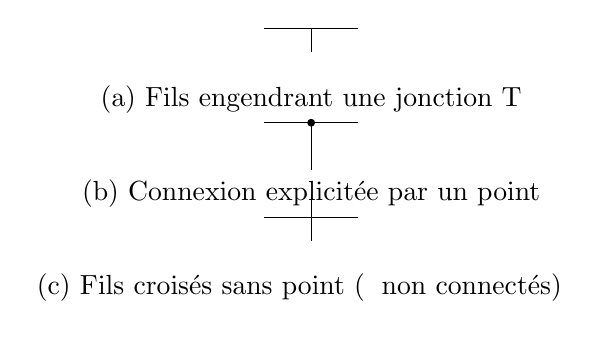
\begin{tikzpicture}[node distance=1.5cm, scale=0.60]

    % Wire junction at a T
    \draw (0,0) -- (2,0);
    \draw (1,0) -- (1,-0.5);
    \node[below] at (1,-1) {(a) {Fils engendrant une jonction T}};

    % Wires connect at a dot
    \draw (0,-2) -- ++(2,0);
    \draw (1,-2) -- ++(0,-1);
    \filldraw (1,-2) circle (2pt);
    \node[below] at (1,-3) {(b) Connexion explicitée par un point};

    % Wires crossing without connecting
    \draw (0,-4) -- ++(2,0);
    \draw (1,-3.5) -- (1,-4.5);
    \node[below] at (0.75,-5) {(c) Fils croisés sans point (\;$\therefore$ non connectés)};

\end{tikzpicture}    
\end{center}

    \paragraph{Circuit de priorité}
    \mbox{}\vspace{0.5em}



\begin{center}
 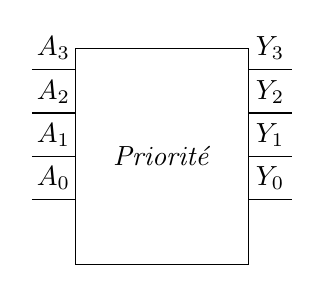
\begin{tikzpicture}[scale=0.55]
    % Draw the box for the priority circuit
    \draw (0,0) rectangle (4,5);
    \node at (2,2.5) {\textit{Priorité}};

    % Draw the input lines and labels
    \draw (-1,4.5) -- (0,4.5) node[midway, above] {\(A_3\)};
    \draw (-1,3.5) -- (0,3.5) node[midway, above] {\(A_2\)};
    \draw (-1,2.5) -- (0,2.5) node[midway, above] {\(A_1\)};
    \draw (-1,1.5) -- (0,1.5) node[midway, above] {\(A_0\)};

    % Draw the output lines and labels
    \draw (4,4.5) -- (5,4.5) node[midway, above] {\(Y_3\)};
    \draw (4,3.5) -- (5,3.5) node[midway, above] {\(Y_2\)};
    \draw (4,2.5) -- (5,2.5) node[midway, above] {\(Y_1\)};
    \draw (4,1.5) -- (5,1.5) node[midway, above] {\(Y_0\)};
\end{tikzpicture}    
\end{center}


\begin{table}[H]
  \centering
  \renewcommand{\arraystretch}{1.5}
  \setlength{\arrayrulewidth}{0.4pt}
  \arrayrulecolor{blue}
  \scriptsize
  \begin{tabular}{|c|c|c|c||c|c|c|c|}
    \hline
    \rowcolor{lightBlue}
    \textcolor{myb}{$A_3$} & \textcolor{myb}{$A_2$} & \textcolor{myb}{$A_1$} & \textcolor{myb}{$A_0$} & \textcolor{myb}{$Y_3$} & \textcolor{myb}{$Y_2$} & \textcolor{myb}{$Y_1$} & \textcolor{myb}{$Y_0$} \\
    \hline
    \hline
    0 & 0 & 0 & 0 & 0 & 0 & 0 & 0 \\
    \rowcolor{lightBlue}
    0 & 0 & 0 & 1 & 0 & 0 & 0 & \textcolor{blue}{1} \\
    0 & 0 & 1 & 0 & 0 & 0 & \textcolor{blue}{1} & 0 \\
    \rowcolor{lightBlue}
    0 & 0 & 1 & 1 & 0 & 0 & \textcolor{blue}{1} & 0 \\
    0 & 1 & 0 & 0 & 0 & \textcolor{blue}{1} & 0 & 0 \\
    \rowcolor{lightBlue}
    0 & 1 & 0 & 1 & 0 & \textcolor{blue}{1} & 0 & 0 \\
    0 & 1 & 1 & 0 & 0 & \textcolor{blue}{1} & 0 & 0 \\
    \rowcolor{lightBlue}
    0 & 1 & 1 & 1 & 0 & \textcolor{blue}{1} & 0 & 0 \\
    1 & 0 & 0 & 0 & \textcolor{blue}{1} & 0 & 0 & 0 \\
    \rowcolor{lightBlue}
    1 & 0 & 0 & 1 & \textcolor{blue}{1} & 0 & 0 & 0 \\
    1 & 0 & 1 & 0 & \textcolor{blue}{1} & 0 & 0 & 0 \\
    \rowcolor{lightBlue}
    1 & 0 & 1 & 1 & \textcolor{blue}{1} & 0 & 0 & 0 \\
    1 & 1 & 0 & 0 & \textcolor{blue}{1} & 0 & 0 & 0 \\
    \rowcolor{lightBlue}
    1 & 1 & 0 & 1 & \textcolor{blue}{1} & 0 & 0 & 0 \\
    1 & 1 & 1 & 0 & \textcolor{blue}{1} & 0 & 0 & 0 \\
    \rowcolor{lightBlue}
    1 & 1 & 1 & 1 & \textcolor{blue}{1} & 0 & 0 & 0 \\
    \hline
  \end{tabular}
\end{table}

    \paragraph{Représentation d'un circuit de priorité}
    \mbox{}\vspace{0.5em}

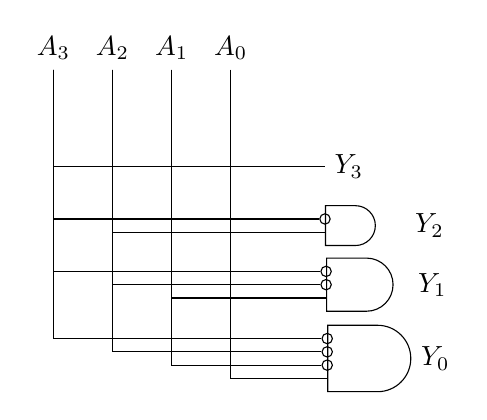
\begin{tikzpicture}[label distance=1mm, scale=0.75]

    \node (x0) at (0,0) {$A_3$};
    \node (x1) at (1,0) {$A_2$};
    \node (x2) at (2,0) {$A_1$};
    \node (x3) at (3,0) {$A_0$};



    \node at ($(x3)+(2,-2)$) (And1) {$Y_3$};
    \node[and gate US, draw, logic gate inputs=nn] at ($(And1)+(0,-1)$) (And2) {};
    \node[and gate US, draw, logic gate inputs=nnn] at ($(And2)+(0.15,-1)$) (And3) {};
    \node[and gate US, draw, logic gate inputs=nnnn] at ($(And3)+(0.15,-1.25)$) (And4) {};


    \draw (x0) |- (And1);
    \draw (x0) |- (And1);
    \draw (And2.input 1) circle (2.5pt);
    
    \draw (x0) |-  ($(And2.input 1)+(-0.1,0)$);
    \draw (x1) |-  (And2.input 2);


    \draw (x0) |-  ($(And3.input 1)+(-0.1,0)$);
    \draw (x1) |-  ($(And3.input 2)+(-0.1,0)$);
    \draw (x2) |-  (And3.input 3);
    \draw (And3.input 1) circle (2.5pt);
    \draw (And3.input 2) circle (2.5pt);


    \draw (x0) |-  ($(And4.input 1)+(-0.1,0)$);
    \draw (x1) |-  ($(And4.input 2)+(-0.1,0)$); 
    \draw (x2) |-  ($(And4.input 3)+(-0.1,0)$);
    \draw (x3) |-  (And4.input 4);
    \draw (And4.input 1) circle (2.5pt);
    \draw (And4.input 2) circle (2.5pt);
    \draw (And4.input 3) circle (2.5pt);

    \draw ($(And2.output) + (0.5,0)$)  node[right] {$Y_2$}; 
    \draw ($(And3.output) + (0.25,0)$) node[right]{$Y_1$};
    \draw (And4.output)  node[right] {$Y_0$};

\end{tikzpicture}


\paragraph{Entrée don't care ou $\mathbb{X}$}
    Ces entrés sont utilisées pour spécifier que la variables possédant le 
    \textit{don't care} n'affecte pas le résultat de la fonction logique.   
    Une file de priorité peut être résumée par la table suivante. 


\begin{table}[H]
  \centering
  \renewcommand{\arraystretch}{1.5}
  \setlength{\arrayrulewidth}{0.4pt}
  \arrayrulecolor{blue}
  \scriptsize
  \begin{tabular}{|c|c|c|c||c|c|c|c|}
    \hline
    \rowcolor{lightBlue}
    \textcolor{myb}{$A_3$} & \textcolor{myb}{$A_2$} & \textcolor{myb}{$A_1$} & \textcolor{myb}{$A_0$} & \textcolor{myb}{$Y_3$} & \textcolor{myb}{$Y_2$} & \textcolor{myb}{$Y_1$} & \textcolor{myb}{$Y_0$} \\
    \hline
    \hline
    0 & 0 & 0 & 0 & 0 & 0 & 0 & 0 \\
    \rowcolor{lightBlue}
    0 & 0 & 0 & 1 & 0 & 0 & 0 & \textcolor{blue}{1} \\
    \rowcolor{lightBlue}
    0 & 0 & 1 & \textcolor{red}{\textit{d}}   & 0 & 0 & \textcolor{blue}{1} & 0 \\
    0 & 1 & \textcolor{red}{\textit{d}} & \textcolor{red}{\textit{d}} & 0 & \textcolor{blue}{1} & 0 & 0 \\
    \rowcolor{lightBlue}
    1 & \textcolor{red}{\textit{d}} & \textcolor{red}{\textit{d}} & \textcolor{red}{\textit{d}} & \textcolor{blue}{1} & 0 & 0 & 0 \\
    \hline
  \end{tabular}
\end{table}


    \paragraph{Contention : signal X }
    Se produit lorsque les portes logiques et les entrées sont telles 
    que la sortie à générer est \textbf{contradictoire}.   


    \begin{center}
        \begin{circuitikz}[label distance=1mm, scale=0.75]
            % Define the NOT gates
            \node[not port] (not1) at (0,0) {};
            \node[not port] (not2) at (0,-2) {};
            \node (jonction) at (1,-1) {};

            % Connect the NOT gates outputs to the same node (contention)
            \draw (not1.out) -| (1,-1) node[above right] {$Y=\mathbb{X}$};    
            \draw (not2.out) -| (1,-1);
            % Connect the NOT gates inputs to the labels
            \draw (not1.in) -- ++(-1,0) node[left] {$A = 1$};
            \draw (not2.in) -- ++(-1,0) node[left] {$B = 0$};
        \end{circuitikz}        
    \end{center}



    \paragraph{Tampon à trois états : signal $\mathbb{Z}$}
    Circuit dans lequel une entrée $\mathbb{E}$ est connecté à une porte tampon et contrôle 
    la \textbf{propagation du signal}. Lorsque l'entrée $\mathbb{E}$ est 
    sous tension haute, la porte agit comme un tampon normal; lorsque l'entrée 
    $\mathbb{E}$ est sous tension basse, la porte produit le signal $\mathbb{Z}$ qui 
    indique que $A$ est \textit{contrôlé}.   

    \begin{center}
        \begin{circuitikz}[scale=0.5]
        % Define buffer gate
        \node[buffer] (buf) at (0,0) {};
        
        % Draw input and output lines
        \draw (buf.in) -- ++(-1,0) node[left] {$A$};
        \draw (buf.out) -- ++(1,0) node[right] {$Y$};
        
        % Draw enable line
        \draw ($(buf.in) + (1, 1)$) -- ++(0,1) node[above] {$E$};
        \end{circuitikz}        
    \end{center}


    \paragraph{Méthodes de Karnaugh}
    Méthode \textbf{graphique}   
    permettant de simplifier les formules de circuits 

    \begin{itemize}
        \item[$\rhd$]   \textbf{Organiser}  les éléments en grille 
            de façon à ce que chaque cellule ne diffère d'une 
            cellule voisine que par \textbf{1 bit}.   
        \item[$\rhd$] Remplir la grille de façon à refléter le 
            \textbf{tableau d'origine}.   
        \item[$\rhd$] \textbf{Grouper} ou entourer les cellules 
            adjacentes qui possèdent un \textbf{1}.   
    \end{itemize}   


    \begin{table}[H]
    \centering
    \footnotesize
    \begin{tabular}{|c|c|c||c|}
    \hline
    \rowcolor{lightBlue}
    \textcolor{myb}{$A$} & \textcolor{myb}{$B$} 
                       & \textcolor{myb}{$C$} 
                       & \textcolor{myb}{$Y$}\\
    \hline
    \hline
    0 & 0 & 0 & \textcolor{blue}{1}   \\ 
    \rowcolor{lightBlue}
    0 & 0 & 1 & \textcolor{blue}{1} \\ 
    \rowcolor{lightBlue}
    0 & 1 & 0 & 0 \\
    0 & 1 & 1 & 0 \\
    \rowcolor{lightBlue}
    1 & 0 & 0 & 0 \\
    1 & 0 & 1 & 0 \\
    \rowcolor{lightBlue}
    1 & 1 & 0 & 0 \\
    1 & 1 & 1 & 0 \\
    \hline
  \end{tabular}
\end{table}        


    \begin{center}
        \begin{karnaugh-map}[4][2][1][$B$][$A$][$C$][$$]
            \minterms{0,4}
            \autoterms[0] 
            \implicant{0}{4}
        \end{karnaugh-map}
    \end{center}


    \begin{center}
        \begin{karnaugh-map}[4][2][1][$B$][$A$][$C$][$$]
          \terms{0}{\tiny{$\overline{A}\cdot\overline{B}\cdot\overline{C}$}}
            \terms{4}{\tiny{$\overline{A}\cdot\overline{B}C$}}
            \autoterms[0]
        \end{karnaugh-map}
    \end{center}
    \textbf{Solution} : considérer les variables qui ne changent pas 
    leurs valeurs entre les cases \textbf{groupés}. Ici, la variable 
    $C$ change de valeur entre le cellule 1 et la cellule 2; 
    elle n'est donc pas considérée dans \textbf{l'équation simplifiée}. 
    Nous avons alors :
    \[Y = \overline{A}\overline{B} \]

    \paragraph{Autre exemple de Karnaugh-map de 3 entrées}
    Parfois, il y a plusieurs \textbf{implicants}. 
    \begin{table}[H]
    \centering
    \footnotesize
    \begin{tabular}{|c|c|c||c|}
    \hline
    \rowcolor{lightBlue}
    \textcolor{myb}{$A$} & \textcolor{myb}{$B$} 
                       & \textcolor{myb}{$C$} 
                       & \textcolor{myb}{$Y$}\\
    \hline
    \hline
    0 & 0 & 0 & 0 \\ 
    \rowcolor{lightBlue}
    0 & 0 & 1 & 0 \\ 
    \rowcolor{lightBlue}
    0 & 1 & 0 & \textcolor{blue}{1} \\
    0 & 1 & 1 & \textcolor{blue}{1} \\
    \rowcolor{lightBlue}
    1 & 0 & 0 & 0 \\
    1 & 0 & 1 & 0 \\
    \rowcolor{lightBlue}
    1 & 1 & 0 & \textcolor{blue}{1} \\
    1 & 1 & 1 & 0 \\
    \hline
  \end{tabular}
\end{table}        


    \begin{center}
      \tiny
        \begin{karnaugh-map}[4][2][1][$B$][$A$][$C$][$$]
            \minterms{1,3,5}
            \autoterms[0] 
            \implicant{1}{3}
            \implicant{1}{5}
        \end{karnaugh-map}
    \end{center}
    \[ Y = \overline{A}B + B\overline{C} \] 


     \paragraph{Autre exemple de Karnaugh-map de 3 entrées}
     Pour les tables de Karnaugh à 4 entrées et plus, les implicants 
     devinnent plus complexes. 

  \begin{table}[H]
    \centering
    \renewcommand{\arraystretch}{1.15}
    \setlength{\arrayrulewidth}{0.4pt}
    \arrayrulecolor{blue}
    \scriptsize
    \begin{tabular}{|c|c|c|c||c|}
      \hline
      \rowcolor{lightBlue}
      \textcolor{myb}{$A$} & \textcolor{myb}{$B$} & \textcolor{myb}{$C$} & \textcolor{myb}{$D$} & \textcolor{myb}{$Y$} 
      \\ \hline
      0 & 0 & 0 & 0 & \textcolor{blue}{1} \\
      \rowcolor{lightBlue}
      0 & 0 & 0 & 1 & 0 \\
      0 & 0 & 1 & 0 &  \textcolor{blue}{1}  \\
      \rowcolor{lightBlue}
      0 & 0 & 1 & 1 & \textcolor{blue}{1} \\
      0 & 1 & 0 & 0 & 0 \\
      \rowcolor{lightBlue}
      0 & 1 & 0 & 1 & \textcolor{blue}{1}  \\
      0 & 1 & 1 & 0 & \textcolor{blue}{1}  \\
      \rowcolor{lightBlue}
      0 & 1 & 1 & 1 & \textcolor{blue}{1} \\
      1 & 0 & 0 & 0 & \textcolor{blue}{1} \\
      \rowcolor{lightBlue}
      1 & 0 & 0 & 1 & \textcolor{blue}{1} \\
      1 & 0 & 1 & 0 & \textcolor{blue}{1} \\
      \rowcolor{lightBlue}
      1 & 0 & 1 & 1 & 0 \\
      1 & 1 & 0 & 0 & 0 \\
      \rowcolor{lightBlue}
      1 & 1 & 0 & 1 & 0 \\
      1 & 1 & 1 & 0 & 0 \\
      \rowcolor{lightBlue}
      1 & 1 & 1 & 1 & 0 \\
      \hline
    \end{tabular}
  \end{table}


  \begin{center}
      \tiny
        \begin{karnaugh-map}[4][4][1][$B$][$A$][$D$][$C$]
            \minterms{0, 2, 5, 6, 12, 13, 8, 9, 10}
            \implicant{2}{6}
            \implicantcorner
            \implicant{12}{9}
            \implicant{5}{13}
        \end{karnaugh-map}
  \end{center}


  \paragraph{Karnaugh-map avec Don't Cares}
  Les \textit{don't care} peuvent complexifier la simplifiation de la 
  fontion à cause du plus grand nombre de \textbf{cas possibles}
  lors du regroupement. 



  \begin{table}[H]
    \centering
    \renewcommand{\arraystretch}{1.5}
    \setlength{\arrayrulewidth}{0.4pt}
    \arrayrulecolor{blue}
    \scriptsize
    \begin{tabular}{|c|c|c|c||c|}
      \hline
      \rowcolor{lightBlue}
      \textcolor{myb}{$A$} & \textcolor{myb}{$B$} & \textcolor{myb}{$C$} & \textcolor{myb}{$D$} & \textcolor{myb}{$Y$} 
      \\ \hline
      0 & 0 & 0 & 0 & \textcolor{blue}{1} \\
      \rowcolor{lightBlue}
      0 & 0 & 0 & 1 & 0 \\
      0 & 0 & 1 & 0 &  \textcolor{blue}{1}  \\
      \rowcolor{lightBlue}
      0 & 0 & 1 & 1 & \textcolor{blue}{1} \\
      0 & 1 & 0 & 0 & 0 \\
      \rowcolor{lightBlue}
      0 & 1 & 0 & 1 & \textcolor{red}{$\mathbb{X}$}    \\
      0 & 1 & 1 & 0 & \textcolor{blue}{1}  \\
      \rowcolor{lightBlue}
      0 & 1 & 1 & 1 & \textcolor{blue}{1} \\
      1 & 0 & 0 & 0 & \textcolor{blue}{1} \\
      \rowcolor{lightBlue}
      1 & 0 & 0 & 1 & \textcolor{blue}{1} \\
      1 & 0 & 1 & 0 & \textcolor{blue}{1} \\
      \rowcolor{lightBlue}
      1 & 0 & 1 & 1 & \textcolor{red}{$\mathbb{X}$} \\
      1 & 1 & 0 & 0 & \textcolor{red}{$\mathbb{X}$} \\
      \rowcolor{lightBlue}
      1 & 1 & 0 & 1 & \textcolor{red}{$\mathbb{X}$} \\
      1 & 1 & 1 & 0 & \textcolor{red}{$\mathbb{X}$} \\
      \rowcolor{lightBlue}
      1 & 1 & 1 & 1 & \textcolor{red}{$\mathbb{X}$} \\
      \hline
    \end{tabular}
  \end{table}

  


  
  % paragraph  (end)


  \begin{center}
      \tiny
        \begin{karnaugh-map}[4][4][1][$B$][$A$][$D$][$C$]
            \minterms{0,2,6, 12, 13, 8,9}
            \terms{3,5,7, 15, 14, 13, 10}{$\mathbb{X}$}
            \implicantcorner
            \implicant{3}{10}
            \implicant{12}{10}
        \end{karnaugh-map}
  \end{center}

  \[ Y = A + \overline{B} \cdot \overline{D} + C \]


  \paragraph{Karnaugh-map de 5 entrées}
  Il faut considérer \textbf{deux} K-map de \textbf{quatre} variables. Par convention, 
  on peut omettre la première variable dans les deux K-map; on considère que la 
  dans la première K-map, la variable irgnorée a une valeur de \textbf{0} et, dans la 2e K-map, 
  elle a une valeur de \textbf{1}. 
  \href{https://www.youtube.com/watch?v=CZPwYZdmMI0&t=417s}{\texttt{Exemple sur Youtube}} 
  Soit la fonction et K-maps correspondantes :  
  \begin{align*}
    f(A, B, C, D, E) = &\sum(0, 1, 2, 4, 5, 6, 10, 13, 
                    \\ &14 18, 21, 22, 24, 26, 29, 30)
  \end{align*}


  \begin{figure}[H]  
    \caption*{\footnotesize{K-map de $BCDE$ en considérant $A = 0$}}
    \begin{center}
        \begin{karnaugh-map}[4][4][1][$C$][$B$][$E$][$D$]
          \terms{0}{1\;\tiny{\textcolor{myp}{0}}}
          \terms{1}{1\;\tiny{\textcolor{myp}{1}}}
          \terms{4}{1\;\tiny{\textcolor{myp}{4}}}
          \terms{5}{1\;\tiny{\textcolor{myp}{5}}}
          \terms{7}{1\;\tiny{\textcolor{myp}{7}}}
          \terms{8}{1\;\tiny{\textcolor{myp}{8}}}
          \terms{9}{1\;\tiny{\textcolor{myp}{9}}}
          \terms{10}{1\;\tiny{\textcolor{myp}{10}}}
          \terms{11}{1\;\tiny{\textcolor{myp}{11}}}
          \terms{2}{0\;\tiny{\textcolor{myp}{2}}}
          \terms{3}{0\;\tiny{\textcolor{myp}{3}}}
          \terms{6}{0\;\tiny{\textcolor{myp}{6}}}
          \terms{12}{0\;\tiny{\textcolor{myp}{12}}}
          \terms{13}{0\;\tiny{\textcolor{myp}{13}}}
          \terms{14}{0\;\tiny{\textcolor{myp}{14}}}
          \terms{15}{0\;\tiny{\textcolor{myp}{15}}}
            \minterms{0, 1, 4, 5, 7, 8, 9, 11, 10}
            \implicant{0}{5}
            \implicant{5}{7}
            \implicant{8}{10}
        \end{karnaugh-map}    \end{center}
  \end{figure}

  \[ \textcolor{myyellow!50}{D\overline{E}} + \textcolor{green}{C\overline{D} \cdot E}   
  + \textcolor{red}{\overline{A} \cdot \overline{B} \cdot \overline{D}}  \]
    


   \begin{figure}[H]
    \caption*{\footnotesize{K-map de $BCDE$ en considérant $A = 1$}}
    \begin{center}
    
      \begin{karnaugh-map}[4][4][1][$C$][$B$][$E$][$D$]
          \terms{0}{0\;\tiny{\textcolor{myp}{16}}}

          \terms{1}{0\;\tiny{\textcolor{myp}{17}}}
          
          \terms{4}{0\;\tiny{\textcolor{myp}{20}}}
          \terms{5}{1\;\tiny{\textcolor{myp}{21}}}
          \terms{7}{1\;\tiny{\textcolor{myp}{23}}}


          \terms{8}{1\;\tiny{\textcolor{myp}{24}}}
          \terms{9}{1\;\tiny{\textcolor{myp}{25}}}
          \terms{10}{1\;\tiny{\textcolor{myp}{26}}}
          \terms{11}{1\;\tiny{\textcolor{myp}{27}}}
          \terms{2}{0\;\tiny{\textcolor{myp}{18}}}
          \terms{3}{0\;\tiny{\textcolor{myp}{19}}}
          \terms{6}{0\;\tiny{\textcolor{myp}{22}}}

          \terms{12}{0\;\tiny{\textcolor{myp}{28}}}
          \terms{13}{0\;\tiny{\textcolor{myp}{29}}}
          \terms{14}{0\;\tiny{\textcolor{myp}{28}}}
          \terms{15}{0\;\tiny{\textcolor{myp}{31}}}
            \minterms{2, 5, 7, 8, 9, 10, 11}
            \implicantedge{2}{2}{10}{10}
            \implicant{5}{7}
            \implicant{8}{10}
        \end{karnaugh-map}    \end{center}
    \caption{}
  \end{figure}


  \[ \textcolor{myyellow!50}{D\overline{E}} + \textcolor{green}{C\overline{D} \cdot E}   
  + \textcolor{red}{A B \cdot \overline{C}}  \]

  \paragraph{Karnaugh-map de 6 entrées}
  \mbox{}\vspace{0.5em}
  \begin{note}{}{}
        On peut utiliser la même approches que la méthode pour entrée, cette fois 
        en considérant \textbf{4} K-map de 4 variables superposées dans un cube 
        tridimensionnel
        \href{https://www.youtube.com/watch?v=LXJXZOqZpGk}{Exemple sur \texttt{Youtube}}
  \end{note}
    \paragraph{Multiplexeur}
    \begin{itemize}
        \item[$\rhd$]  $2^n$ lignes d'entrées 
        \item[$\rhd$]  $2^n$ N lignes de sélections 
        \item[$\rhd$]  $2^n$ Une seule sorties $Y$  
    \end{itemize}
    Possède deux implémentations secondaires, soit (1) \textbf{portes logiques}
    et (2) \textbf{tampons} à trois états. 
    \end{multicols*}

\end{document}
